\subsection{The effect of $K$-way majority voting on \texttt{LINC} and \texttt{CoT}}
\label{appendix:k_way}

In all our experiments, we use 10-way majority voting, inspired by prior work which found that Chain-of-Thought prompting benefited therefrom \cite{wang2023self}.
However, one might wonder how robust the performance gains seen with \texttt{LINC} are to the precise value of $K$. 
Figure~\ref{fig:k_way} thus shows, for each model equipped with either \texttt{LINC} or \texttt{Chain-of-Thought}, how the accuracy on FOLIO varies with $K \in \{1, 2, 3, \dots, 10\}$.
We note that, generally speaking, \texttt{LINC} makes good use of increased values of $K$. This is especially true for the weaker models; these are more prone to generating syntactically invalid FOL expressions, which cause the solver to return an Error. Taking the majority vote over many samples thus lessens the risk of predicting Error, which is of course always the wrong label.
Notably, our results do not indicate that \texttt{CoT} benefits from majority voting in this domain.
Future work is needed to establish how this relates to the findings in the previously mentioned prior work.

\begin{figure}[bh]
    \centering
    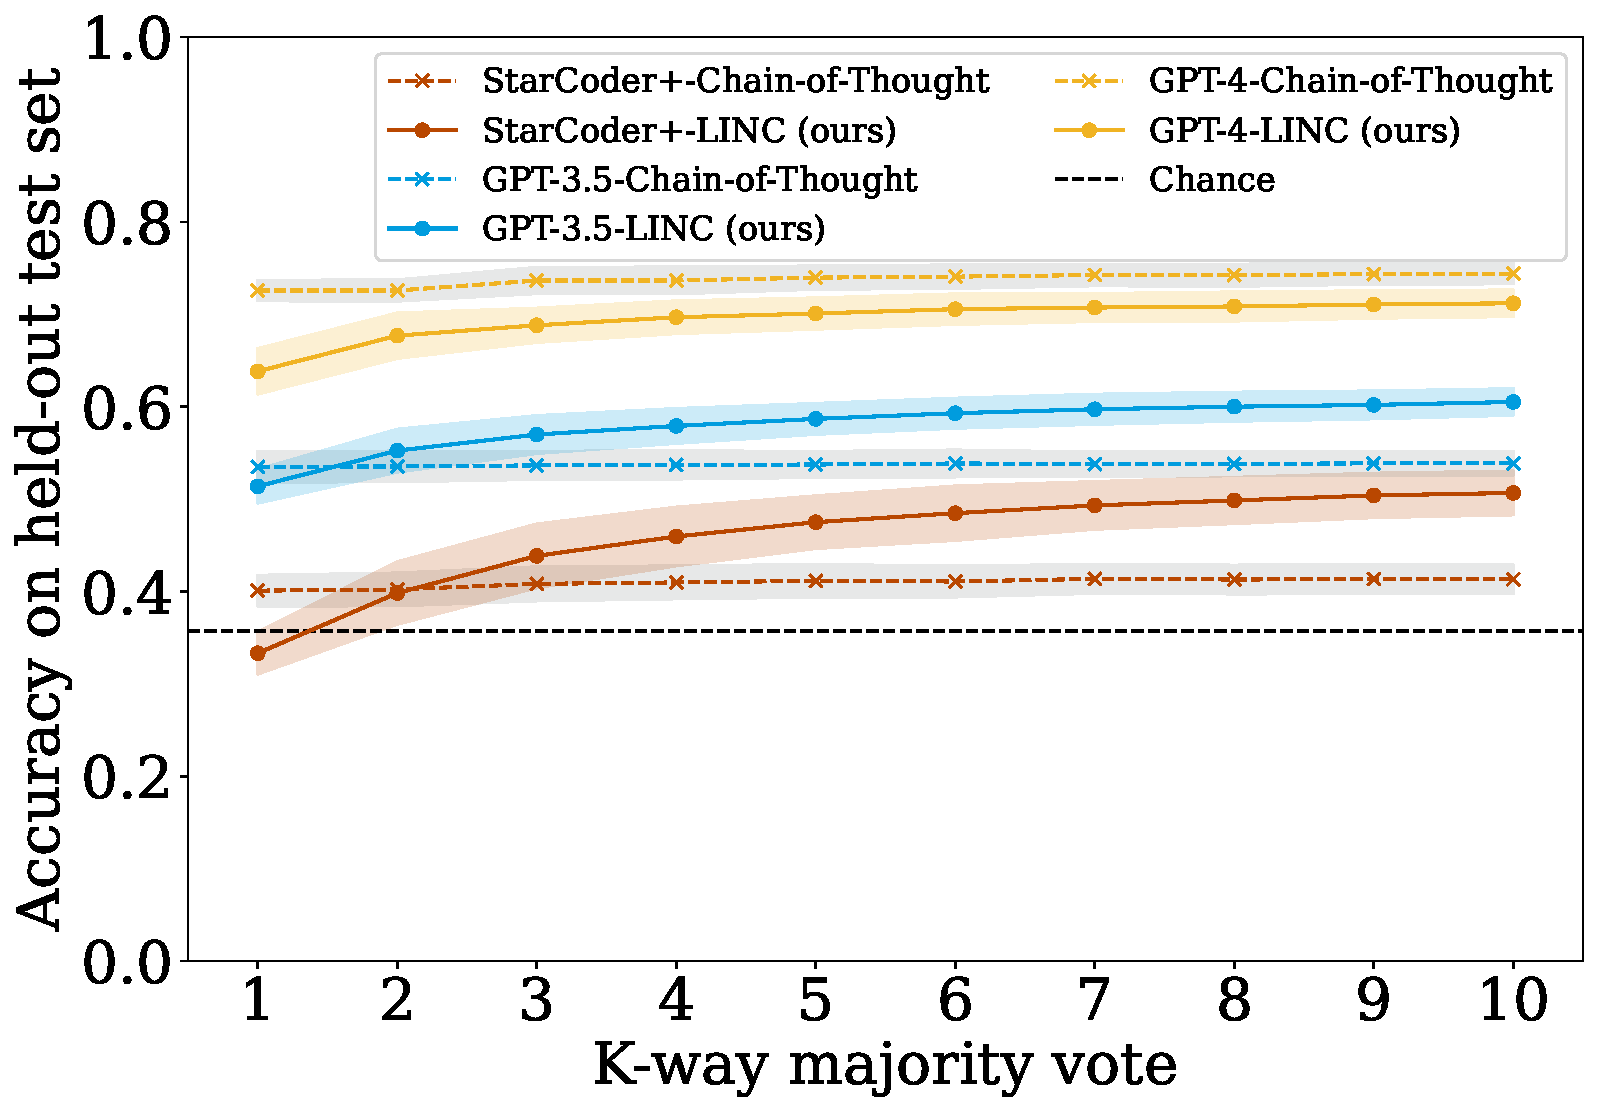
\includegraphics[width=0.45\textwidth]{figures/kmaj/folio_kmaj.pdf}
    \caption{Accuracy on FOLIO per value of $K$ (Appendix~\ref{appendix:k_way}). Shaded areas are $\pm 1$ standard deviation over 1000 bootstrapped samples. Note that increasing $K$ benefits \texttt{LINC} (solid lines; shading in color) but not \texttt{CoT} (dashed lines; shading in gray) in our experiments on this dataset.}
    \label{fig:k_way}
\end{figure}
